\documentclass[12pt]{article}
\usepackage{currothesis}
\usepackage[left=1.5in, right=1.5in, top=1in, bottom=1in]{geometry}
\usepackage{fontspec}
\setmainfont{Adobe Caslon Pro}
\usepackage{layout}
\usepackage[]{amsmath}
\usepackage{amssymb}
\usepackage{ragged2e}
\usepackage{graphicx}
\usepackage{cite}
\usepackage{booktabs}
\usepackage{tikz}
\usepackage{caption} 
\captionsetup[table]{skip=10pt}
\usetikzlibrary{matrix,chains,positioning,decorations.pathreplacing,arrows}

\DeclareMathOperator*{\argmin}{arg\,min}

\usepackage{titlesec}

\setcounter{secnumdepth}{4}

\titleformat{\paragraph}
{\normalfont\normalsize\bfseries}{\theparagraph}{1em}{}
\titlespacing*{\paragraph}
{0pt}{3.25ex plus 1ex minus .2ex}{1.5ex plus .2ex}

\def\toclevel@paragraph{4}
\setcounter{tocdepth}{4}
\pagestyle{plain}
\setlength{\marginparwidth}{1in}

\newcommand\tline[2]{$\underset{\text{#1}}{\text{\underline{\hspace{#2}}}}$}

\begin{document}

% Title page
\thispagestyle{empty}
\begin{center}
\Large

THE COOPER UNION\\
ALBERT NERKEN SCHOOL OF ENGINEERING

\vspace{1in}

{
\LARGE
Alternative Architectures for \\Generative Adversarial Networks

}

\vspace{1in}

by

Christopher Curro

\vspace*{\fill}

A thesis submitted in partial fulfillment\\
of the requirements for the degree of\\
Master of Engineering

\vspace{1in}

September 2016

\vspace{1in}

Professor Sam Keene, Advisor

\end{center}

% Signature Page
\newpage
\thispagestyle{empty}
\begin{center}
\Large
THE COOPER UNION FOR THE \\ADVANCEMENT OF SCIENCE AND ART

\vspace{0.5in}

ALBERT NERKEN SCHOOL OF ENGINEERING

\vspace{1in}

\justify

This thesis was prepared under the direction of the Candidate's Thesis Advisor
and has received approval. It was submitted to the Dean of the School of
Engineering and the full Faculty, and was approved as partial fulfillment of
the requirements for the degree of Master of Engineering.

\raggedright

\vspace{1in}

\hfill \tline{Dean, School of Engineering \hfill Date}{3in}

\vspace{1in}

\tline{Prof. Sam Keene, Thesis Advisor \hfill Date}{3in}


\end{center}

\newpage
\pagenumbering{roman}
\setcounter{page}{1}

\newpage

Ack

\newpage

Abstract


\newpage

\tableofcontents

\newpage

\listoffigures

\newpage

Table of Nomenclature

\clearpage
\setcounter{page}{1}
\pagenumbering{arabic}

\fontsize{12pt}{24pt}\selectfont 
\section{Introduction}
\subsection{Machine Learning at Large}
% explain ML basics
Machine learning involves the use of computer algorithms to make decisions based on training data. Generally, this falls into categorizing input data (classification) or determining a mathetmatical function to determine a continuous output given an input (regression). Popular classification examples include recognizing handwritten digits as well as determining whether an image contains a cat or a dog. An example of a regression problem is determining the temperature given a set of input features (humidity, latitude, longitude, date, etc.).

Problems where training data contain input data vectors as well as the correct output vectors (targets) are known as supervised learning problems. Training a model to denoise audio where noise was introduced to the clean audio would be a supervised learning problem. On the other hand, training a model to denoise audio where the underlying clean signal is not known is an unsupervised learning problem. Different loss (objective) functions and neural network architectures can be exploited to accomplish denoising without the clean data.

For the purposes of this thesis, we use machine learning to determine an underlying nonlinear function that removes noise from time slices of audio (i.e. regression). These slices can then be pieced back together through overlap-add resynthesis. To clarify, this is a general linear model that maps an input noisy audio vector $y[n]=x[n]+N[n]$ to $\tilde{x}[n]$, a target denoised audio vector, where $x[n]$ is the underlying clean signal and $N[n]$ is the additive background noise.

\subsubsection{Regression}
A classical regression technique is linear regression, where one or more independent variables $x_{i}$ are used to determine a scalar dependent variable $y$. The case of a single independent variable $x$ is known as simple linear regression. More formally, for $k$ independent variables, we would like to determine a weight vector $\vec{w}$ and bias vector $\vec{b}$:

\begin{align}
y_i &= w_{1}x_{i1} + \cdots + w_{k}x_{ik} + b_{i}, \qquad i=1\ldots ,n \\
\vec{y} &= \vec{x^T}\vec{w} + \vec{b}
\end{align}

where the rows of $x^{T}$ are the example input observations and $\vec{y}$ and $\vec{b}$ are column vectors.

By extension, the case of linearly estimating a vector output giving a vector input is known as a generalized linear model. A canonical example would be estimating a sine wave $x[n]$ over some number of $N$ samples given noisy samples $y[n]=x[n]+N[n]$.


% \subsubsection{Overfitting and Curse of Dimensionality}


% \subsubsection{Loss functions and Regularization}


% \subsubsection{Gradient Stuff?}


\subsection{Neural Networks}
% Basic explanation of NN
In this thesis, we deal only with feed-forward neural networks, which are essentially directed acyclic graphs (DAG) for computation. In other words, information only moves through the network in one direction. An example neural network is shown in Figure \ref{fig:nn}.

\begin{figure}[!ht]
\centering
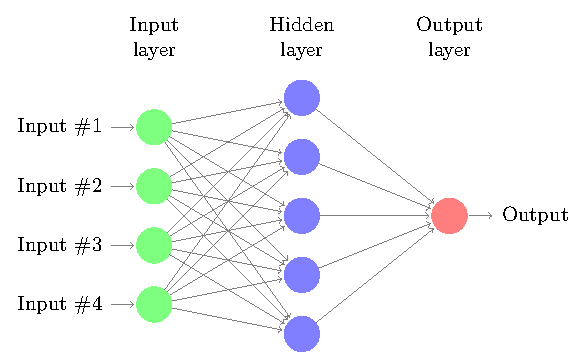
\includegraphics[width=.8\textwidth]{neural-network-texexample-net}
\caption[Example neural network]{An example neural network. There are 4 input variables, 1 hidden layer with 5 neurons, and 1 output variable. Source: http://www.texample.net/tikz/examples/neural-network/}
\label{fig:nn}
\end{figure}

The connections in a neural network can be represented by linear combinations of the input variables with learned weights $\vec{w}$. \cite{bishop} Unlike standard linear models however, neural networks apply a nonlinear activation $f(\cdot)$ at the output of each neuron. The circle nodes in a neural network diagram can be thought of as the sum of the linear combinations of the connection edges and the application of the bias and activation function. Therefore, a hidden neuron $z_{j}$ in a network with $N$ input variable nodes, $M$ hidden nodes, and $K$ output nodes takes on the value

\begin{equation}
z_j = f(a_j)
\end{equation}

where the activiation $a_j$ is given by

\begin{equation}
a_j = \sum_{i=1}^{N} w_{ji}^{(1)}x_i + w_{j0}^{(1)}
\end{equation}

The connection values $w_{ji}$ are referred to as weights, and the scalars $w_{j0}$ are referred to as biases. Note that the superscripted numbers refer to the Then, the output $y_{k}$ is given by

\begin{equation}
y_k = g(a_k)
\end{equation}

where the output activation $a{k}$ is given by

\begin{equation}
a_k = \sum_{j=1}^{M} w_{kj}^{(2)} z_j + w_{k0}^{(2)}
\end{equation}

We are free to choose activation functions, which we will discuss later. However, note that at the output, the function $g(\cdot)$ is often an identity for regression problems and a sigmoid $\sigma(\cdot)$ for classification problems.

Often, the weights and biases are grouped into a weight vector $\vec{w}$. In other words, similar to the linear models described earlier, a neural network is a nonlinear function of input variables $\{x_i\}$ to output variables $\{y_k\}$ where the parameters of the function are learned via training techniques.

\subsubsection{Dense Layer}

Described in the previous section, we refer to a dense layer as a fully connected neural network, in which no interconnections between neurons are missing at each layer. Dense layers can be prone to overfitting. However, as we mention later, overfitting is not an immediate concern for the purposes of this thesis.

\subsubsection{De-noising Autoencoder}

An autoencoder is normally an abstraction of neural networks in which an encode function $\vec{Z}=f(\vec{X})$ and a decode function $\hat{\vec{X}}=g(\vec{Z})$ are learned to learn a lower-dimensional representation of some input $\vec{X}$. \cite{stow} A de-noising autoencoder is a supervised process whereby the clean input is first corrupted by some stochastic process $\vec{Y}=u(\vec{X})$. In other words, the neural network input would be a noisy input $Y$, and the network would try to learn weights such that the network output $\vec{\hat{X}}$ approximates the clean input $\vec{X}$. Another way to frame it is that your network is learning the inverse function of the noise process $u(\vec{x})$.

% \subsubsection{Convolutional Layer}



\subsubsection{Network Training}

In order to train a neural network, we must update the weights such that we minimize a loss function, often some kind of sum-of-square error function. \cite{bishop} Often, a stochastic gradient descent (SGD) approach is taken to determine the weights that minimize the loss function.



% \subsubsection{Regularization}



\subsubsection{Choice of Activation Function}

The most common activation functions used are the logistic sigmoid function and the hyperbolic tangent. \cite{liu2014experiments} The logistic sigmoid function is given by

\begin{equation}
g(x) = \dfrac{1}{1+\exp{(-x)}}
\end{equation}

Note that the sigmoid function has an output on the range $(0,1)$. The hyperbolic tangent function (tanh) is given by

\begin{align}
g(x) &= \dfrac{\sinh{x}}{\cosh{x}}\\
&= \dfrac{\exp{(x)}-\exp{(-x)}}{\exp{(x)}+\exp{(-x)}}\\
&= \dfrac{1-\exp{(-2x)}}{1+\exp{(-2x)}}
\end{align}

Note that the hyperbolic tangent function has an output on the range $(-1,1)$.

Generally, our choice of nonlinearity should be chosen such that the expected range of desired output matches the nonlinearity's. In the case of audio de-noising, different activations can be chosen depending on the input format. For example, time-domain audio frames are often processed with a digital floating point representation on the range of $[-1,1]$. In such a case, the hyperbolic tangent might be appropriate. On the other hand, if we were working with magnitude spectra of an audio signal, we would use a linearity with an output range of $[0,\infty]$.

Recently, a more popular activation function which has in use is the rectified linear unit (ReLU). \cite{glorot2011deep} The ReLU is defined by the following:

\begin{equation}
g(x) =
    \begin{cases}
        \hfill 0 & \text{if $x < 0$}\\
        \hfill x & \text{if $x \ge 0$}
    \end{cases}
\end{equation}

In other words, $g(x)=\max{(0,x)}$. This function satisfies the range of output we expect for magnitude spectra. In terms of gradient calculations, the zero derivative for negative input values of $x$ can cause nodes to not be activated, potentially leading to gaps in information at the output and slower training time. To combat this, variations of the ReLU are used which have small, non-zero gradients for negative input values. For example, leaky ReLU's are defined by

\begin{equation}
g(x) =
    \begin{cases}
        \hfill 0.01x & \text{if $x < 0$}\\
        \hfill x & \text{if $x \ge 0$}
    \end{cases}
\end{equation}

Advantages of ReLU's include better gradient propagation as well as fast computation and sparse representation. Some disadvantages include non-differentiability at $x=0$. Also, depending on use case, sparse representation might not be desired.

\subsubsection{Minibatch Training}

Historically, neural networks were trained one example at a time (online) or in a batch (all examples at once). \cite{wilson2003general} For the online approach, the network weights are updated after gradients are calculated and backpropagated for each training example. On the other hand, the batch approach accumulates average gradients for all examples and then updates the network weights. The batch approach might approximate the true gradients better than the online approach, but the online approach tends to have faster training time and convergence. \cite{wilson2003general} This is because with an online approach, the network is less likely to get stuck in a local minimum.

Minibatch training has become more popular recently. Serving as a midway point between the two approaches, minibatch training exposes the network to a small number of examples and then accumulates gradients and updates the network weights. The trend toward minibatch training comes at a time where parallel computing resources are easily accessible.


\subsubsection{Batch Normalization}

Batch normalization is a technique that helps to speed up training time and convergence. Batch normalization accumulates learned statistics of the network to help achieve loss convergence more quickly. More formally, an input minibatch $x$ is normalized by the following:

\begin{equation}
y = \dfrac{x-\mu}{\sqrt{\sigma^{2}+\epsilon}}\gamma + \beta
\end{equation}

\cite{ioffe2015batch}. During training, the minibatches are normalized to zero-mean, unit-variance and transformed by parameters $\gamma$ and $\beta$. At inference time, the learned parameters are instead used, which are made up of the average statistics from training.

Batch normalization prevents activations from saturating from widely varying input minibatches. This allows us to use faster learning rates and be less careful about how to initialize our parameters. \cite{ioffe2015batch}

\subsection{Generative Models}
\subsubsection{Generative models at large}
\subsubsection{Generative adversarial networks}
\subsubsection{Deep convolutional generative adversarial newtorks}
\subsubsection{Additional techniques for traning generative adversarial networks}

\section{System Description}
\subsection{Energy distance matching}
\subsection{Kernel based moment matching}
\subsection{Convolutions with holes}
\subsection{Style Loss term}
\newpage

\nocite{*}
\fontsize{12pt}{16pt}\selectfont 
\bibliography{bib}{}
\bibliographystyle{IEEEtran}

\end{document}
